\section{Analysis}\label{sec:analysis}

A number of parameters can be tweaked to change the patch matching and storage, and different choices may be appropriate for different applications and performance requirements (both quantitative and qualitative). These parameters include the size of the input images, the size and shape of the patches extracted, the extraction strategy (non-overlapping vs overlapping patches), the sampling strategy used to seed the dictionary, the similarity metric and thresholds used to compare patches, as well as the parameters required for indexing and retrieving patch matches (approximate nearest neighbors). Here we discuss some of the parameter choices made and the experiments that lead up to these choices. Other possible choices are discussed in Sec.\ref{sec:futureext}.

Our quantitative performance metrics involve examining how the patch dictionary size grows with the addition of new images to the database (the growth function and rate) and the compression ratio per image (viewed as a distribution over compression ratios and summarized as the average compression ratio). Qualitative evaluations involve determining whether a human can spot compression artifacts and how salient they are in the images. The authors of this paper manually examined images reconstructed from the dictionary patches. A crowdsourced evaluation strategy involving Amazon's Mechanical Turk may be appropriate for larger-scale studies, but was beyond the scope of this paper.

There will always be a trade-off between compression benefits (storage - patch dictionary size, speed - image reconstruction time) and reconstruction quality. For many computer vision tasks including scene recognition (and thus retrieval), imperfect reconstructions with artifacts may not be a problem as long as the overall scene structure does not change. For instance, \cite{tiny_images} has shown that with images of pixel dimension 32x32, humans are already able to achieve over $80\%$ scene and object recognition rate. See fig.\ref{fig:badrecon} for a demonstration of an image that has serious reconstruction artifacts, but when down sampled (to a thumbnail), they become insignificant, and thus do not necessarily impair visual recognition.

 \begin{figure}
%\hspace{-25mm}
\centering
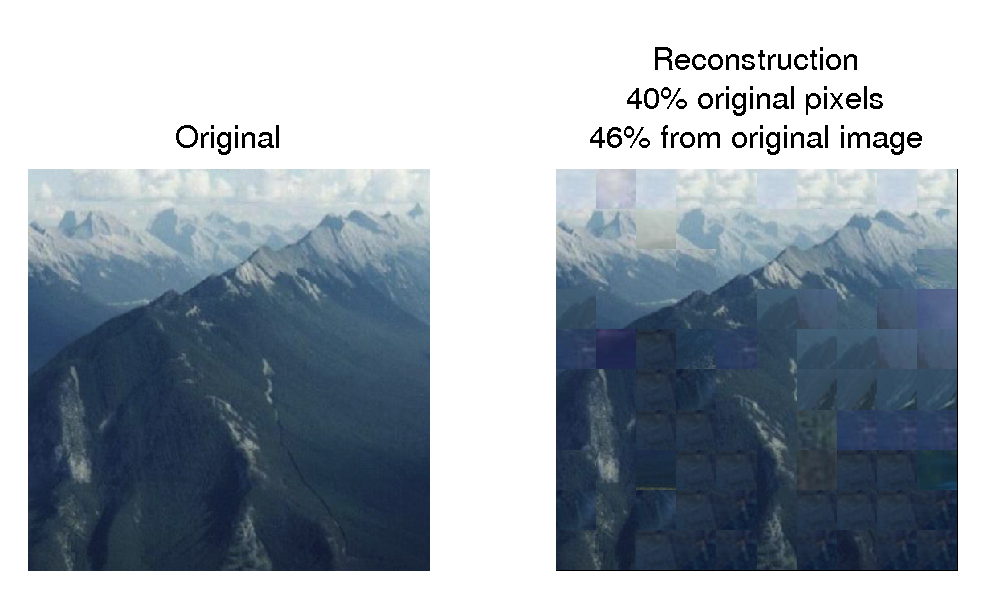
\includegraphics[width=1\linewidth]{Figures/184.png}
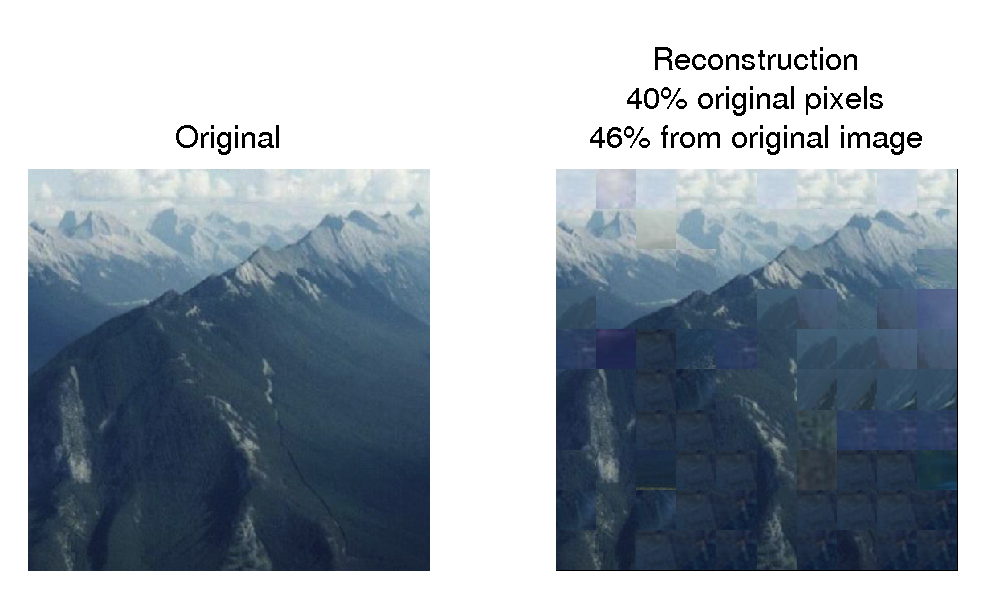
\includegraphics[width=0.5\linewidth]{Figures/184.png}
\caption{For demonstration purposes only, we choose a large patch size and low similarity threshold. Under these parameters, the original image is reconstructed to take up only $40\%$ of its original size (in pixels). The $60\%$ of the patches that have been replaced come either from the same image ($46\%$ of them), or from other images (the remaining $64\%$). Notice that when the size of the image and its reconstruction are halved, the artifacts already become visually insignificant, and would not impair a scene recognition or search task. }
\label{fig:badrecon}
\end{figure}

 \begin{figure}
%\hspace{-25mm}
\centering
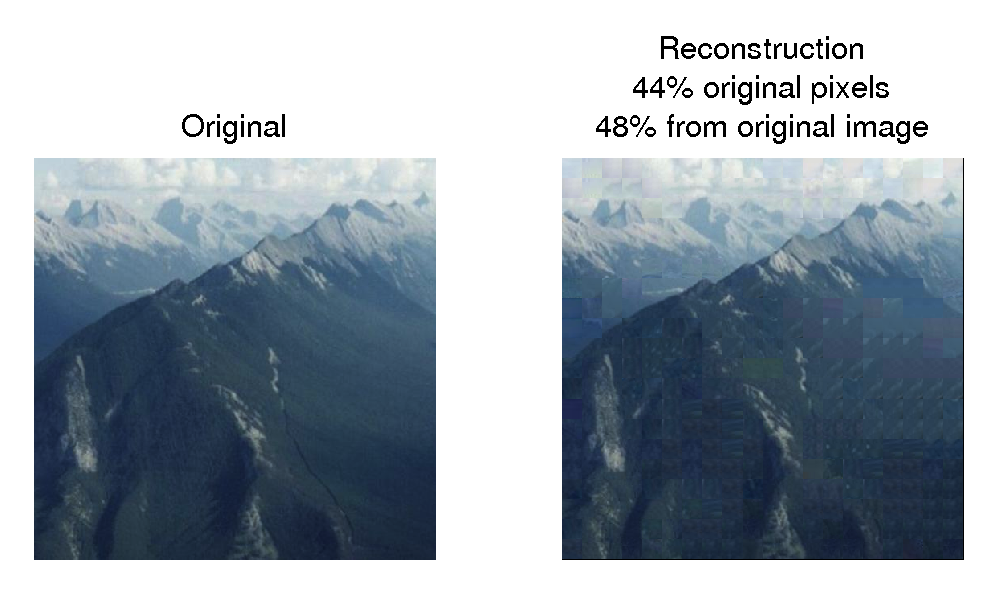
\includegraphics[width=1\linewidth]{Figures/184_25.png}
\caption{Compare this image reconstruction, computed with a dictionary of $25\times 25$ pixel patches with the reconstruction in fig.\ref{fig:badrecon}, computed with $50\times 50$ patches. In both cases, a similar threshold is used (scaled to the patch size, as discussed in sec. \label{sec:simthresh}) but the visual artifacts are less noticeable because smaller patches have less contained structure, and are more likely to be homogenous in appearance.}
\label{fig:patchsize}
\end{figure}


%\subsection{Quality Metrics}\label{ssec:qual-met}
%There are many possible formulations of these quality constraints; we detail those that we considered for this paper in section TODO.  Beyond mathematical metrics, subjective methods are also interesting to consider for formulating the quality constraints; one could imagine a scenario in which image quality is assessed by humans through a crowdsourced system, perhaps using an engine such as Amazon's Mechanical Turk TODO: cite.  We consider such subjective similarity metrics outside the scope of this paper and focus on the mathematical metrics for now.

%We wish to construct a database that trades off minimizing the amount of required space with maximizing read and write speeds of the data.

\subsection{Patch Size}
\label{sec:patchsize}

TODO(Zoya,Andrew): tradeoffs for patch size

At larger patch granularities, each patch contains more image structure, and thus the probability that another patch contains the same or similar image content decreases with the number of pixels in a patch. At larger patch granularities it becomes increasingly harder to find matching patches in the patch dictionary, and the closest matching patches for textured regions might introduce artifacts (see fig.\ref{fig:patchsize}). At the same time, patches that are too small do not offer as efficient a compression strategy. We must balance the costs of storing pointers to patches for each image in our database, as well as all the patches themselves, against the costs of storing the images in their original form. This calculation is investigated further below. 

%In the extreme case, a patch is equal to one pixel, so the probability of an identical color patch is $\frac{1}{255^3}$, assuming 3 color channels. This value is multiplied by itself as many times as there are pixels in a patch to find an identical patch. For our application, we are interested in similar patches, rather than identical ones (see sec.\ref{sec:simthresh}), and so this probability is higher but bounded by this value, and similarly scales with patch size. 

\subsubsection{Cost Evaluation}

Assume for now that we choose to store $p$ patches in our auxiliary table.  In practice, we choose $p$ to be a function $p \colon Function \to \mathds{N}$ which maps from our similarity metric to a number of patches to store.  Assume also that each patch is square and composed of $n^2$ pixels, where $n$ is a user defined parameter.  We further assume that each pixel requires 3 bytes to store  and that each pointer is 8 bytes (a standard integer for a 64-bit system).  Under this "image only" scheme, in the case where we have $i$ images, the cost $c_i$ to store all the images in our database is:

\begin{equation}
	c_i(i, m) = 3  i  m^2
\end{equation}

In the case where we store pointers to patches, we have two tables: one table to store pointers to image patch exemplars, and a second table to store the exemplar data themselves.  Under this "patch pointer"scheme, in the case where we have $i$ images and $p$ patches, the cost $c_p$ to store all the images in our database is:

\begin{equation}
	c_p(i, p, m, n) = 8 i (\frac{m}{n})^2 + 3  p  n^2
\end{equation}.

The first term is the cost of storing the pointer data, while the second term is the cost of storing the patch exemplars themselves.

Given these two equations, for a fixed $m$ and $n$, we can easily see that our compressive scheme becomes more space-efficient when:

\begin{equation}
	p < \frac{m^2 * (3*n^2 - 8) * i}{3*n^4}
\end{equation}

As long as we choose a similarity threshold such that new image patches get added at a rate that guarantees this inequality is satisfied, our compressive method of image storage will save space.

\subsection{Sampling strategies}

A patch dictionary can be built up incrementally, adding new patches as new images are added to the database. A potential problem with this approach is that image reconstruction quality will tend to decrease with the order in which images are added, such that images added to the database earlier will tend to have more patches that correspond to them (see Fig.\ref{fig:sampStrategy} for an example). A strategy with a more even distribution of reconstruction quality over images involves starting with a batch of images, and seeding the dictionary by randomly sampling patches from a set of images from the batch. This is the strategy we employ. 

 \begin{figure}
%\hspace{-25mm}
%\centering
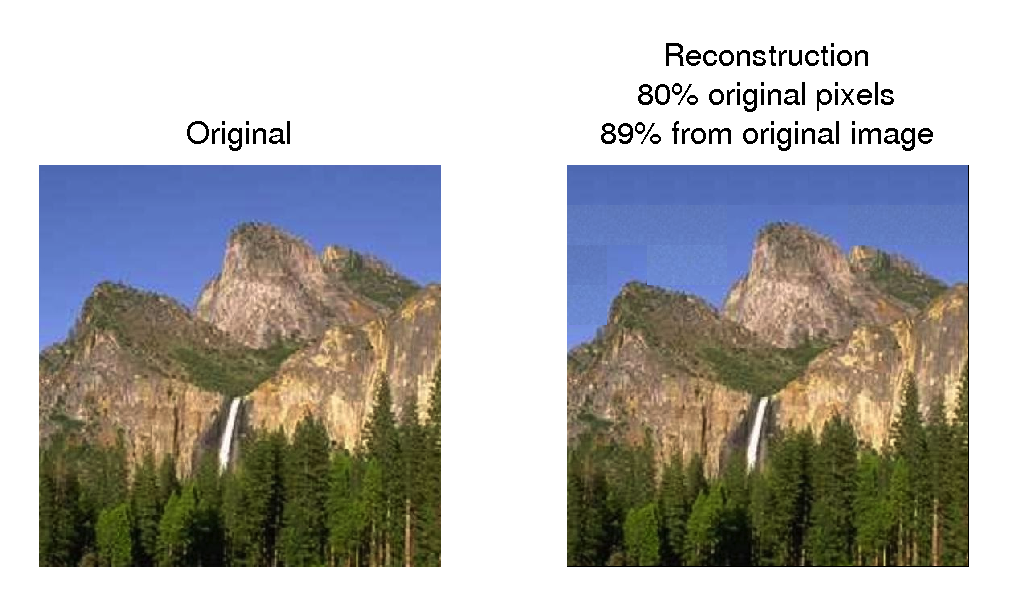
\includegraphics[width=1\linewidth]{Figures/009.png}
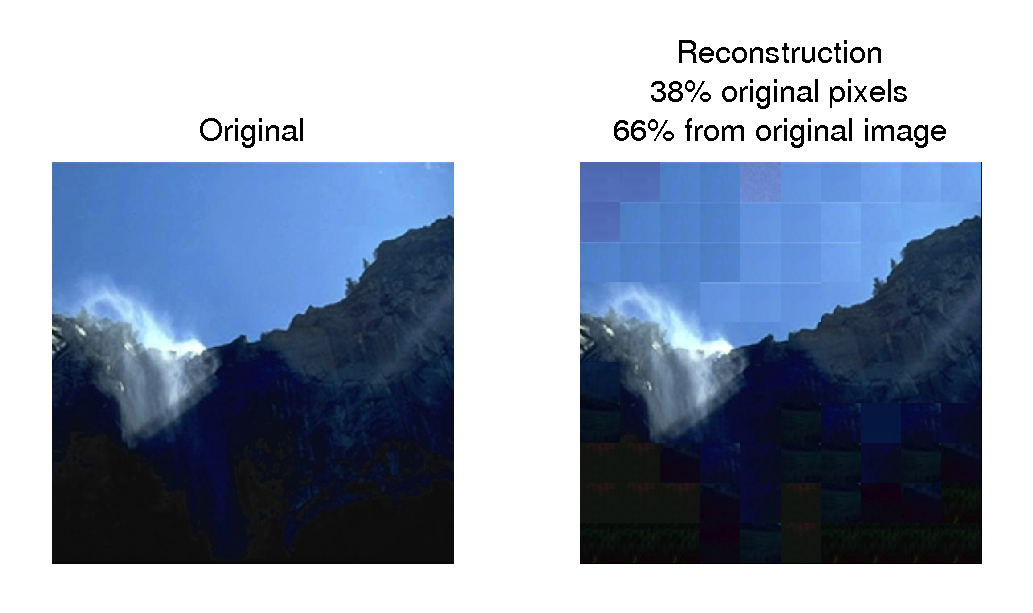
\includegraphics[width=1\linewidth]{Figures/014.png}
\caption{Example of a biased patch dictionary construction strategy, leading to non-uniformity in image reconstruction quality. Images added to the database earlier (top row) are better reconstructed (due to more patch samples in the database) than images added later (bottom row), constrained to be constructed out of patches added initially. The sky pixels in the image added later are borrowed from sky pixels of other images ($44\%$ of the pixels in this image come from other images, compared to only $11\%$ in the image on the first row). Note: here we use a very low patch similarity threshold and large patch size for demonstration purposes only, to emphasize the artifacts created.}
\label{fig:sampStrategy}
\end{figure}


\subsection{Similarity Function}
\label{sec:simthresh}

Many image (more specifically, patch) similarity functions are possible, each with its own distinct set of parameters that can be tweaked for the required application. Because we are dealing with patches of a size specifically chosen to increase within-patch homogeneity, we do not consider cases of patches containing objects (the most we expect is an object boundary or simple texture), and thus do not need to consider complex image similarity functions (like SIFT matching, spatial relationship-preserving functions, etc.). We can constrain ourselves to color similarity, and split a patch $P_i$ into 3 color channels: $P_i(1), P_i(2), P_i(3)$. 

Then we consider two patches $P_i$ and $P_j$ similar when, given $n\times n$ patches, all of the following are true:
\begin{align*}
\frac{1}{n^2}||P_i(1) - P_j(1)||^2 < T_1 \\
\frac{1}{n^2}||P_i(2) - P_j(2)||^2 < T_2 \\
\frac{1}{n^2}||P_i(3) - P_j(3)||^2 < T_3
\end{align*}

The $\frac{1}{n^2}$ term allows us to normalize for patch size, so that the threshold values chosen becomes independent of patch size. Here we constrain the average similarity value of all the pixels to fit a threshold, whereas it is possible to have alternative constraints (whereby the maximal pixel difference, or the variance of the pixel differences, or some other quantity does not exceed a threshold).

Note additionally that if instead, we fix a single threshold for the sum of the Euclidean differences in the 3 color channels: 
\begin{displaymath}
\frac{1}{n^2}[||P_i(1) - P_j(1)||^2 + ||P_i(2) - P_j(2)||^2 + ||P_i(3) - P_j(3)||^2] < T
\end{displaymath}
then the similarity in one color channel may compensate for the difference in another, producing skewed results (see fig.\ref{fig:colProblem}).

Multiple color channels $P_i(1), P_i(2), P_i(3)$ are possible, but we choose to work in the (CIE)LUV color space, which is known to be more perceptually uniform than the standard RGB color space~\cite{kekre2012performance}. Additionally, our formulation makes it possible to impose separate similarity thresholds on each of the color channels ($T_1,T_2,T_3$). However, for simplicity, we set $T_1=T_2=T_3=T$.

\subsection{Similarity Threshold}

Choosing a threshold $T$ requires weighing the quantitative benefits of compression with the qualitatively poorer image reconstructions. We ran a number of experiments, varying the threshold, and quantitatively and qualitatively examining the results. In fig. \ref{fig:perfGraphs} we plot a few small experiments (with 200 images) for demonstrative purposes. The images were $500\times 500$ pixels, and the patch size was $25\times 25$. We chose this patch size due to the discussion in \ref{sec:patchsize}. Below we consider a number of quantitative indicators for patch compression. 

In the set of graphs in the first column of fig. \ref{fig:perfGraphs}, we plot in blue the dictionary size against the number of images added to the database. We compare this to the total number of patches that would have been stored if no compression scheme was utilized (red dotted line). We can see that for all choices of threshold, the size of the patch dictionary grows slower than the total number of patches that would need to be added if all images were stored along with their original patches. The gap between the blue and red dotted lines is a measure of the storage savings. As the threshold becomes more stringent, the blue line approaches the red dotted line. Note additionally that as the threshold becomes smaller, patches are more likely to be reused from the same image than from other images when compressing an image, because only patches from the same image will be similar enough from other patches from this image.

The second column of fig. \ref{fig:perfGraphs} contains histograms indicating how many images contributed different amounts of new patches to the patch dictionary. When the threshold is very small (as in the histogram in the last row) more of the images contribute most of their patches (380-400 new patches added to the patch dictionary per image). Note additionally that the small number of images that is contributing 0 new patches to the dictionary accounts for the $10\%$ duplicates that are present in the SUN database (more about this in sec. \ref{sec:apps}).

The third column of fig. \ref{fig:perfGraphs} contains an insertion history: for each image inserted into the database, we track how many of its patches were added to the patch dictionary. We can see that as the patch similarity threshold decreases, most images contribute most of their pixels. This provides similar information to the histogram (which is merely the cumulative), but allows us to monitor any temporal changes. The spikes to 0 in this graph are indicative of duplicate images, and are discussed in sec. \ref{sec:apps}.

In the final column of fig. \ref{fig:perfGraphs}, we see a sample image reconstruction. We can see that the reconstruction quality increases, and visual artifacts decrease, as the similarity threshold decreases (becomes more stringent). At some point in the middle, the reconstruction is already indistinguishable from the original, but with significant database compression benefits. Thus, for further analysis we consider the threshold $T=8$ (recall that this is per color channel, and is independent of patch size).
%Thus, given two patches $P_i$ and $P_j$, we can measure their similarity in a given color channel by taking the Euclidean distance of the color values across all the pixels. 

%where a patch is a collection of pixels, each of which is defined to be a triplet of integer values, assuming a 3-D color space. For a patch $P_i$, let us define its 3 color channels to be: $P_i(1), P_i(2), P_i(3)$.

 \begin{figure}
%\hspace{-25mm}
%\centering
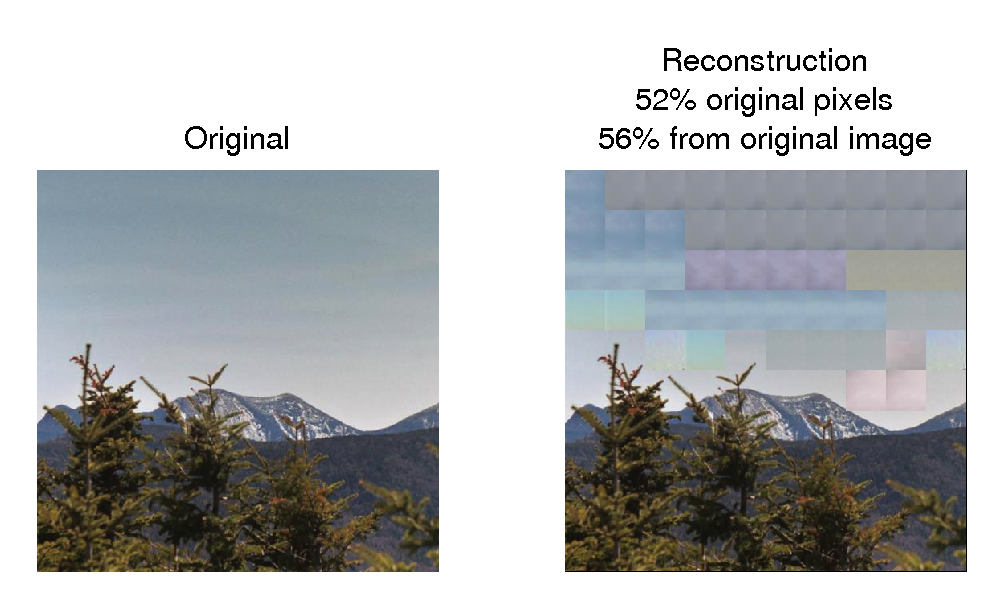
\includegraphics[width=1\linewidth]{Figures/197.png}
\caption{This is what happens when we do not separately constrain each of the color channels to match. We have patches that match in terms of general hue (average of the color channels), but are the wrong color and produce visible visual artifacts.}
\label{fig:colProblem}
\end{figure}

 \begin{figure*}
%\hspace{-25mm}
%\centering
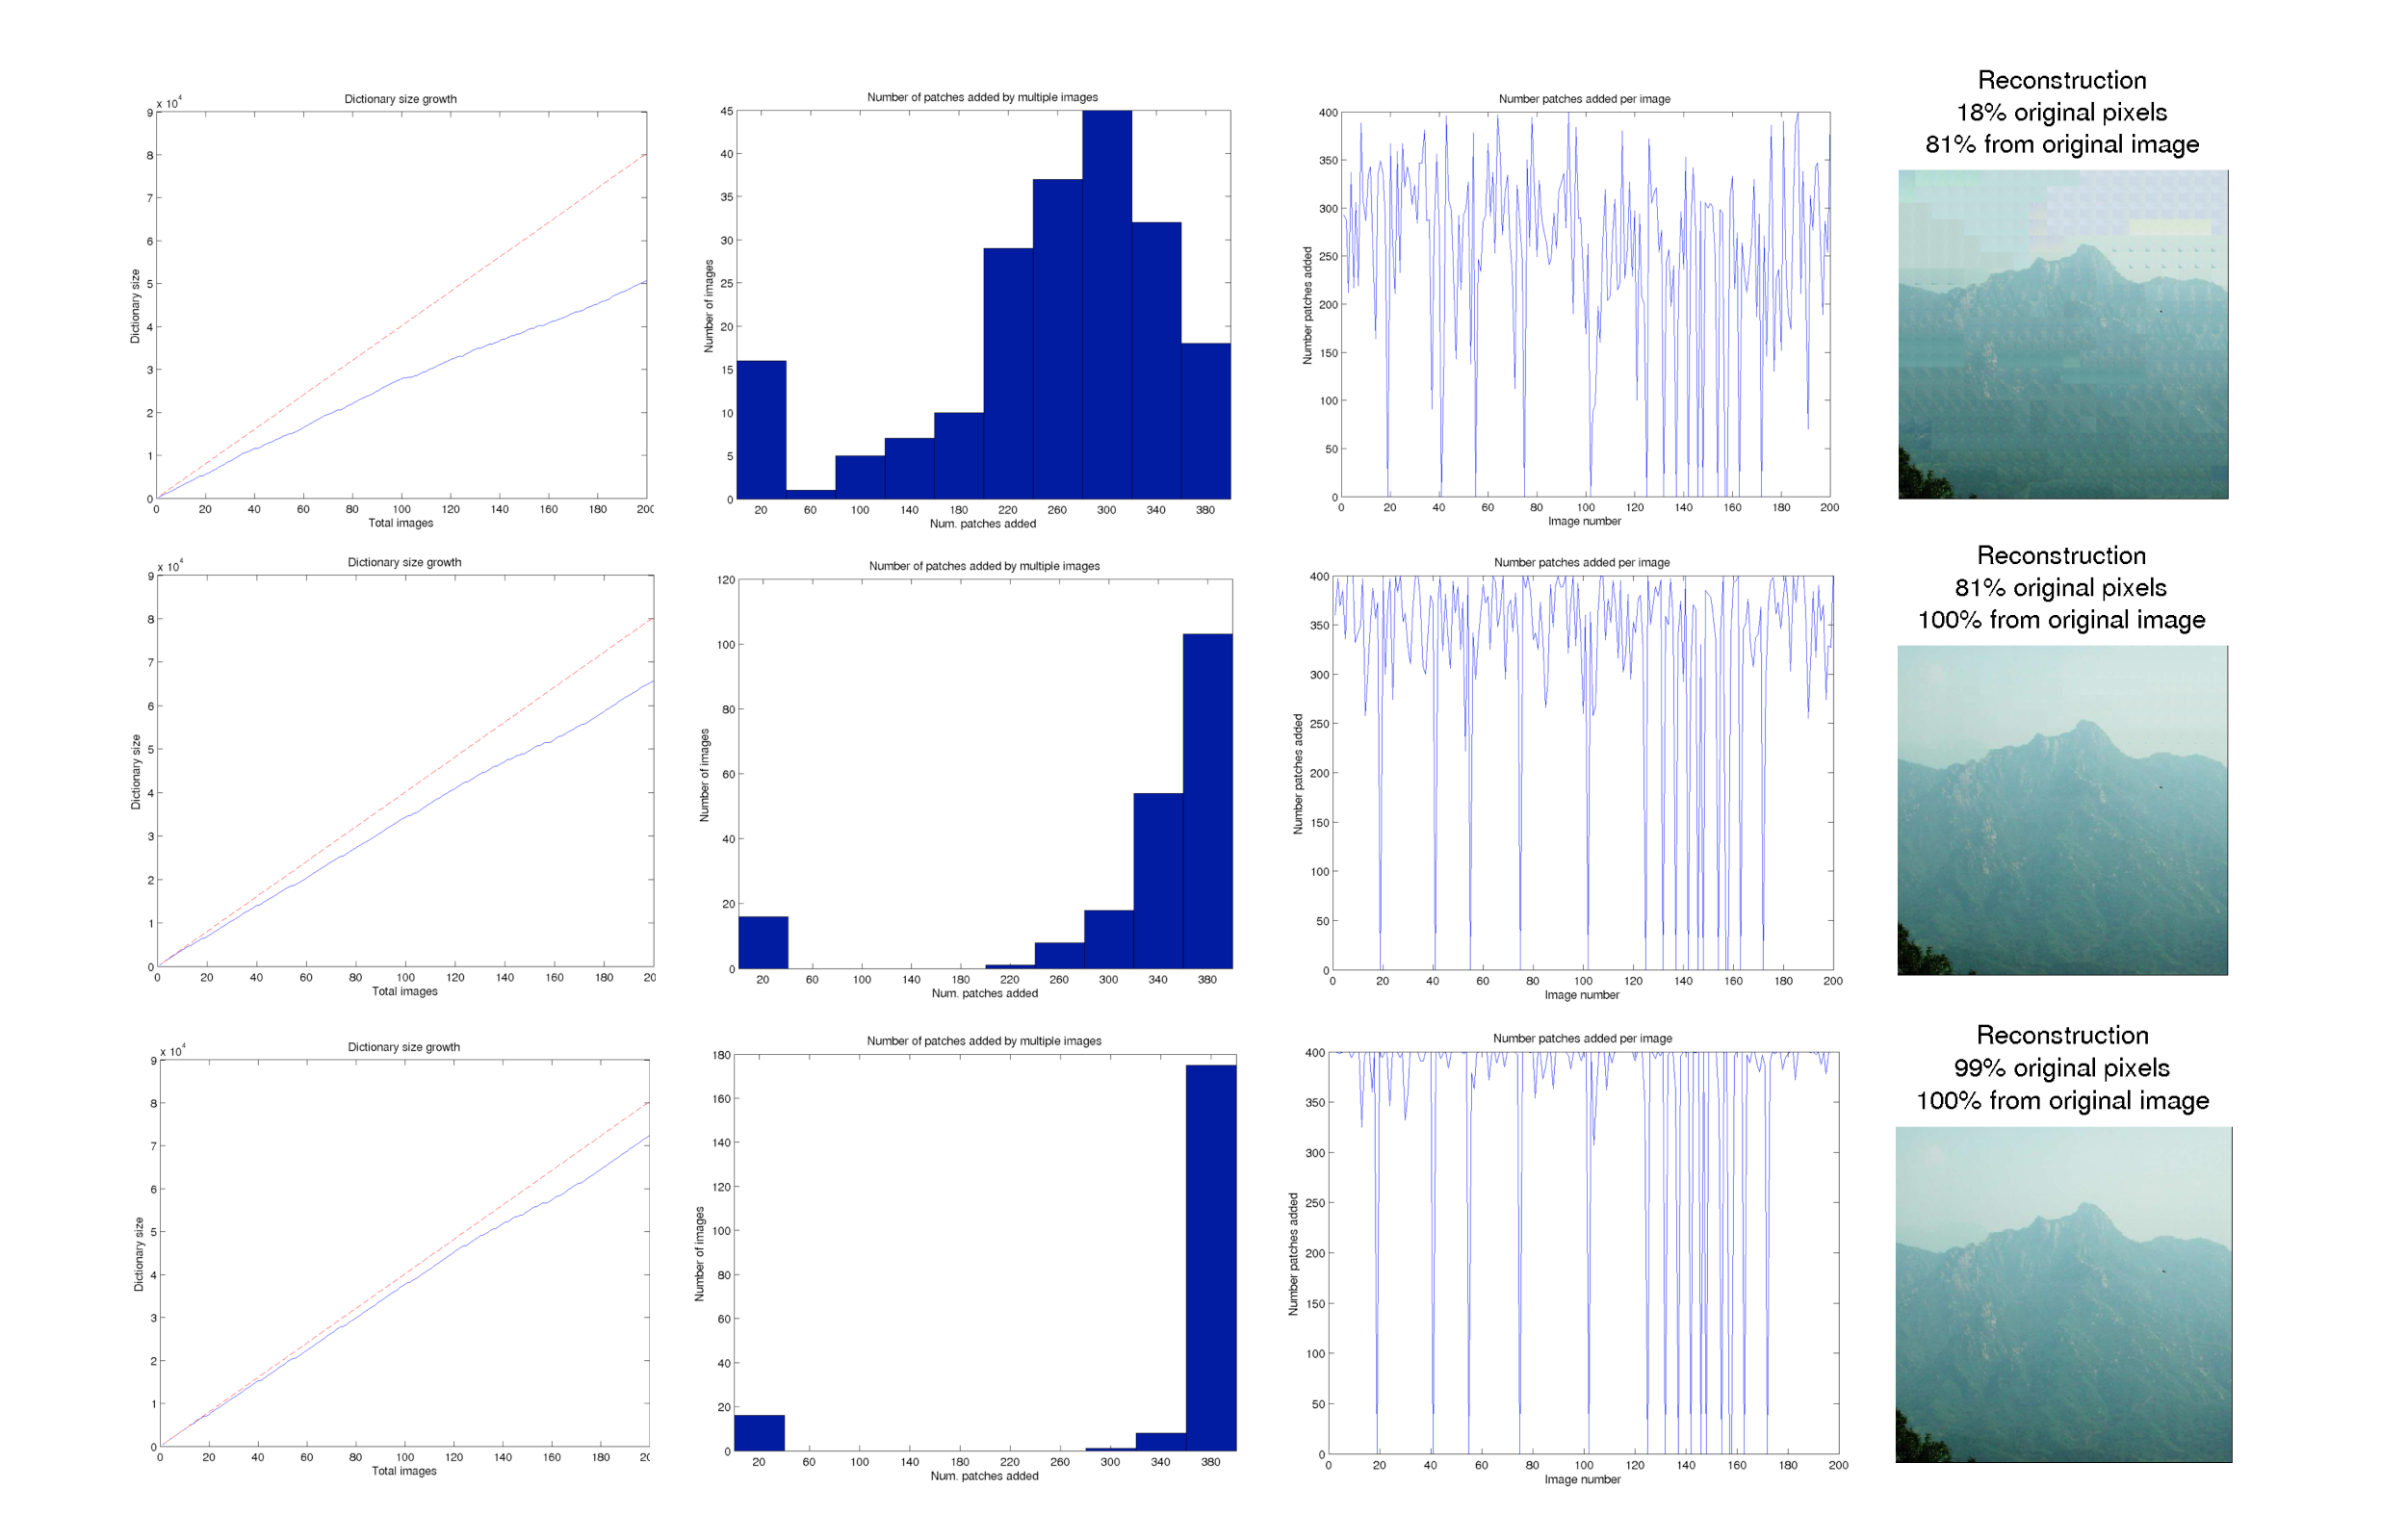
\includegraphics[width=1\linewidth]{Figures/perfGraphs_25.pdf}
\caption{Quantitative and qualitative results obtained by varying the patch similarity threshold, $T$, while extracting $400$ patches from each image. In the first row, $T=80$, the dictionary size is 50,822 patches, and the average compression per image is $36.73\%$. In the second row, $T=8$, the dictionary size is $65,794$ patches, and the average compression per image is $18.09\%$. In the third row, $T=0.8$, the dictionary size is $72,445$ patches, and the average compression per image is $9.80\%$.}
\label{fig:perfGraphs}
\end{figure*}

\subsection{Growing the Database}

In the preceding sections, we determined that for an image sized $500\times 500$, a $25\times 25$ patch size with a $T=0.8$ patch similarity threshold is appropriate since compression savings are properly balanced against artifacts introduced during image reconstruction. For further experiments, we scale down the image size to $100\times 100$ and the patch size to $5\times 5$, accordingly, maintaining the patch:image ratio. Note that the similarity threshold still applies as it is independent of patch size. The reduction in image size allows us to consider larger experiments on databases of image thumbnails. 

In fig. \ref{fig:bigsize} we consider the growth of the patch dictionary as we add 2K images to our database. We add images from different categories, and observe a slight change in dictionary growth rate for every new category added. Although there is some variation across categories, the overall compression is $18.95\%$ per image, demonstrating generalization across categories.

 \begin{figure}
\hspace{-5mm}
%\centering
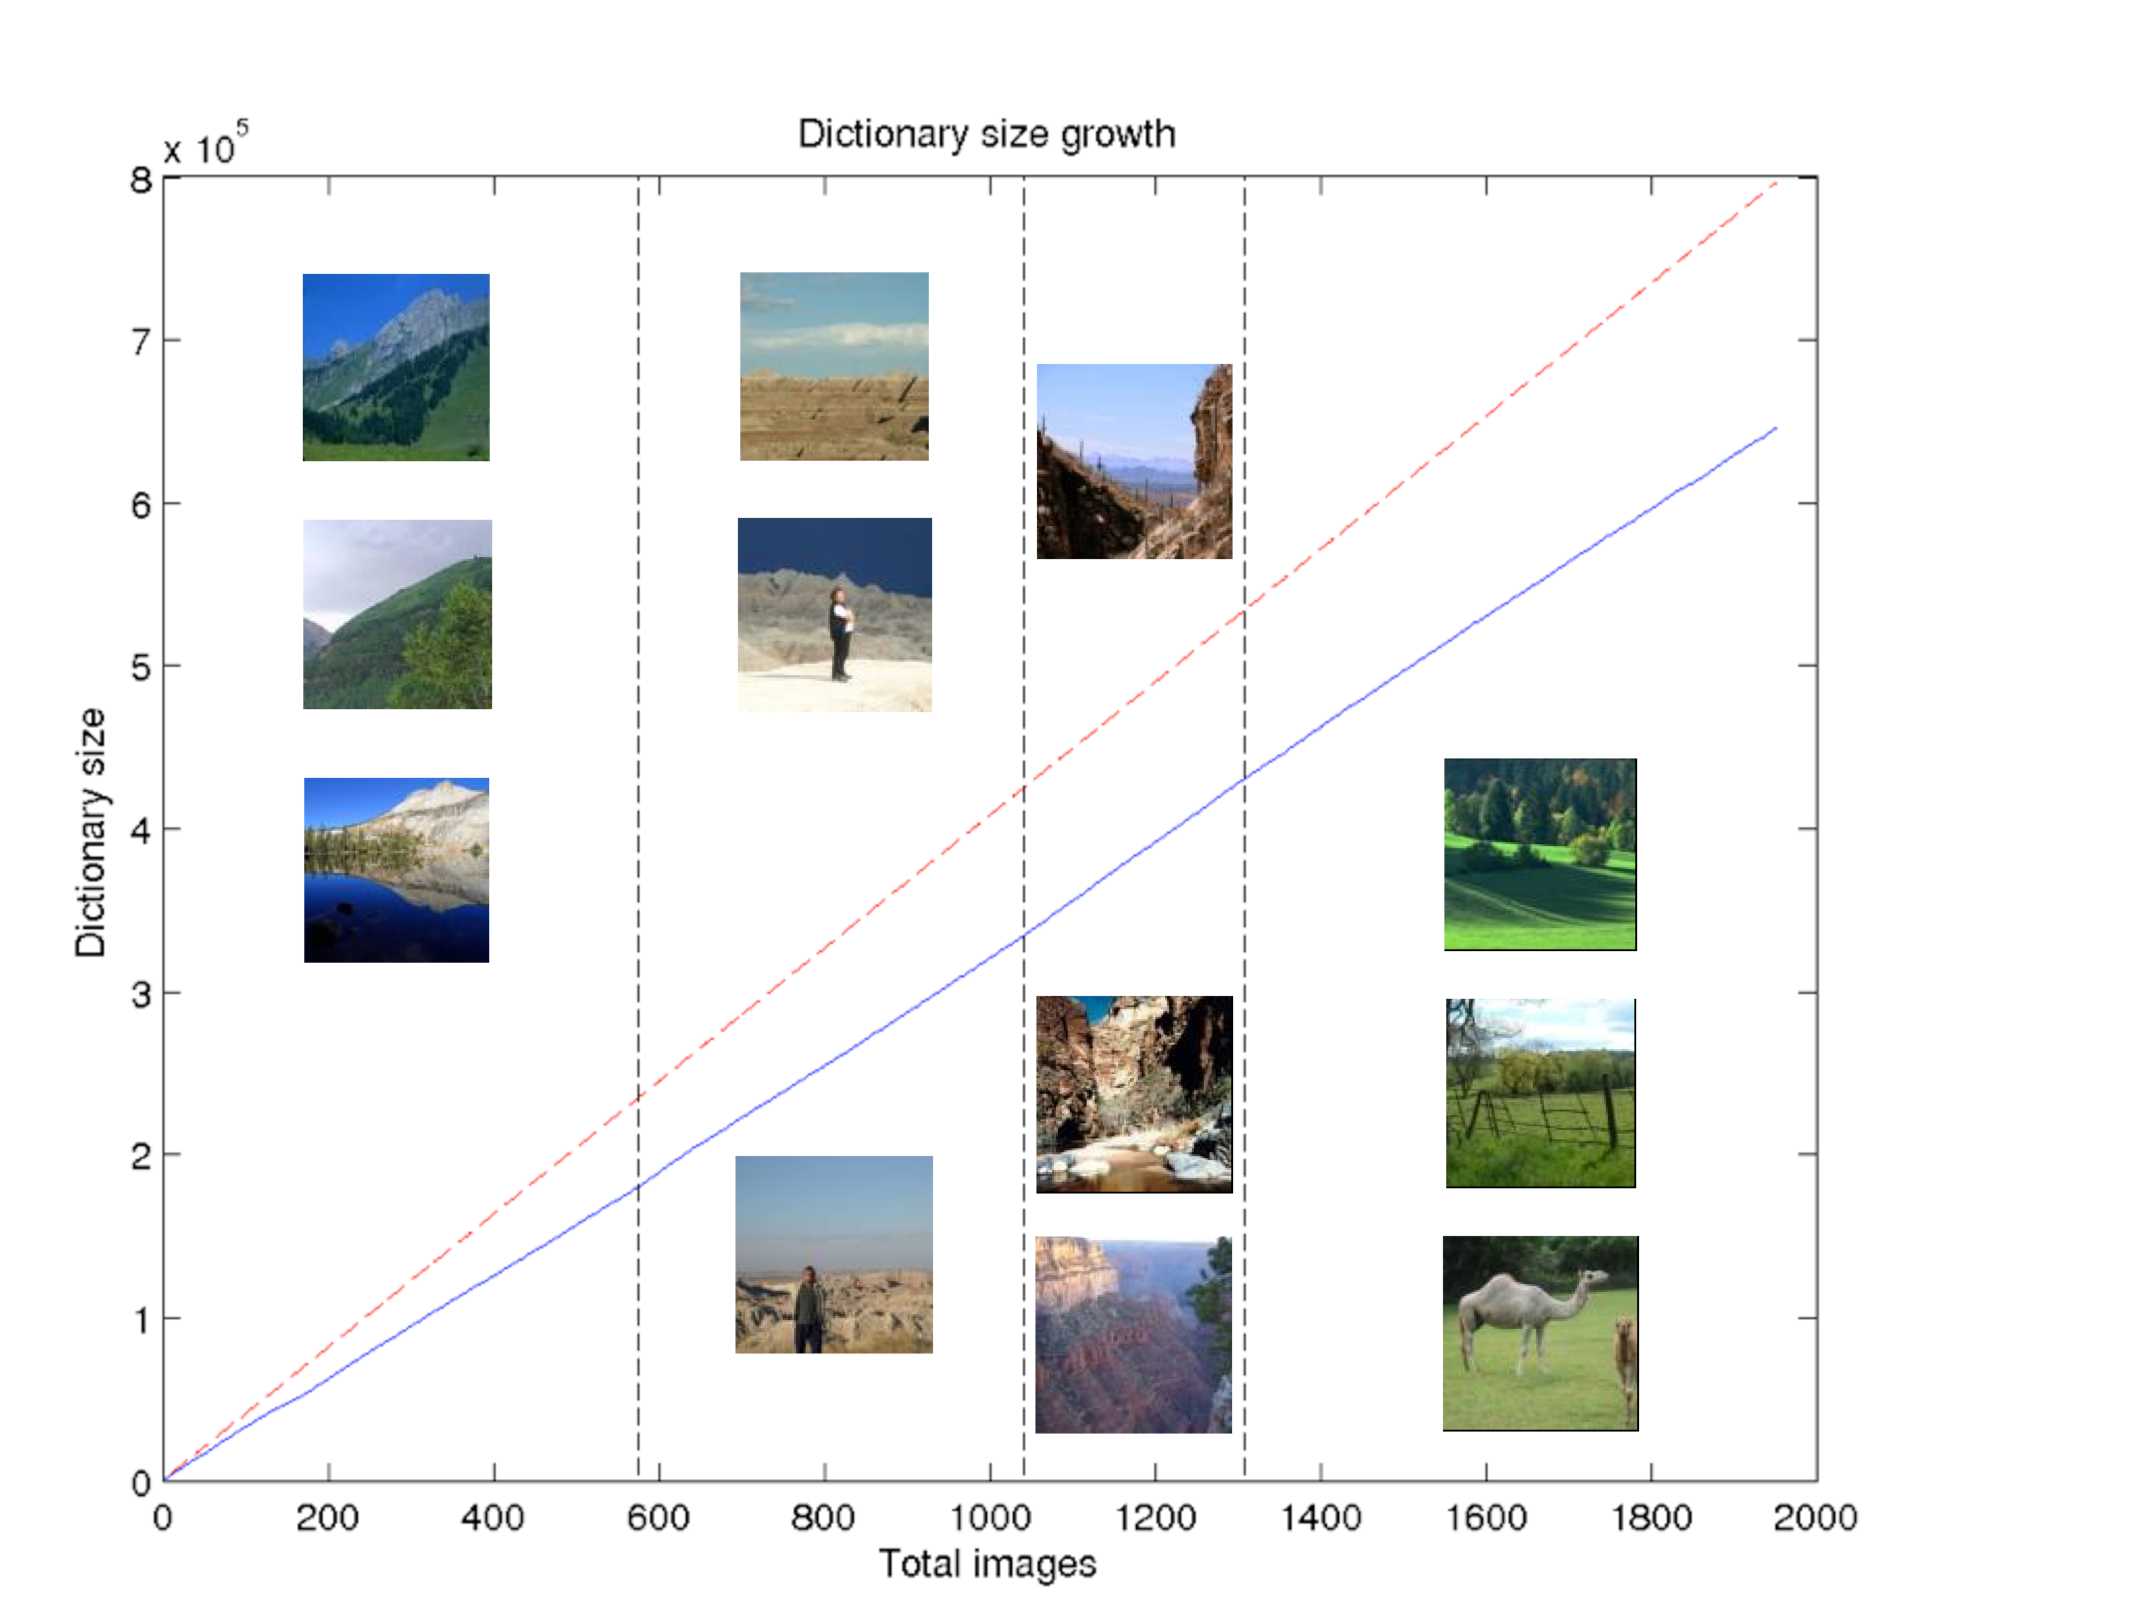
\includegraphics[width=1.3\linewidth]{Figures/multiscenes.pdf}
\caption{A patch dictionary constructed from $5\times 5$ patches from $100\times 100$ images, with a $T=0.8$ patch similarity threshold, obtains an average compression of $18.95\%$ per image. The average number of new patches added per image is $330.70$ with a total dictionary size of $645,534$ patches representing 1952 images. The dotted lines mark the addition of new image categories, (left to right) mountain (with dictionary growth rate 312.96, equivalent to compression of $21.76\%$ per image), badlands (growth rate 330.50, compression $17.38\%$), canyon (growth rate: 360.61, compression $9.85\%$), and pasture (growth rate: 334.11, $16.47\%$). A few image samples from the 4 categories are included.}
\label{fig:bigsize}
\end{figure}

\subsection{Image Type}

TODO: Zoya will add experiments on different scene types

Not all image content is amenable to the same type of compression. For some types of images, particularly where there is a lot of spatial structure (e.g. indoors scenes with objects and parts), compression artifacts are much more noticeable and thus similarity thresholds should be more stringent. An interesting extension that is beyond the score of this paper would be to have a content-aware similarity threshold (self-adjusting to content type such as indoor vs outdoor/natural).
